\documentclass[20 pts]{article}
\usepackage{xeCJK}
\usepackage{amsfonts}
\usepackage{amssymb}
\usepackage{amsmath}
\usepackage{bm}
\setCJKmainfont{SimSun}
\title{Review of Deterministic Interleavers}
\author{Kwame Ackah Bohulu}
\date{25-05-2017}
\begin{document}
\maketitle


\section{Introduction}
Since the discovery of Turbo codes in 1993 a lot of research has been done to further understand how they perform so well. It has been shown that the interleaver plays a very important role in the overall performance of the Turbo code, which is the reduction in the number of low-weight codewords present in the Turbo code through a process called spectral thinning[1]. For large frame sizes, deterministic interleavers are preffered as it is possible perfom interleaving and de-interleaving operations via algorithms instead of storing large interleaver tables.[3]A high error floor is usually present in turbo codes. This can be adjusted in a number of ways, including increasing the free distance of the turbo code whiles maintaining its multiplicity for a fixed interleaver size[1]. In this document, a review of the simplest deterministic interleavers are given. Methods on how to improve their distance properties are also explored.

\section{Block Interleavers and Linear Interleavers}
The simplest deterministic interleaver are the block interleaver and the deterministic interleaver[3]. A block interleaver is a deterministic interleaver definded by a rectangular matrix of size $N=m\times n$. The input bits are written row-wise and read column-wise. The index mapping function of a block interleaver is defined in (1) below[2]

$$\Pi_{\mathfrak{B}_N} \equiv ni + \lfloor l/m\rfloor \mod {N},		0\leq i < N.$$
The index mapping function of a linear interleaver is defined by (2) below

$$\Pi_{\mathfrak{L}_N} \equiv ki + v \mod {N},		0\leq i < N.$$
where $k$ is a fixed integer which is relatively prime to N and v is a fixed integer.

It is noted that the linear interleaver ''linearizes'' the $\lfloor ・\rfloor$ portion of (1). 
Block and Linear interleavers are both based on linear congruence and therefore essentially have the same properties. For example in block interleavers,two elements seperated by a constant $t\mod {N}$ in an input sequence  almost always map to an output sequence with corresponding elements seperated by a fixed constant $tn\mod{n}$ whiles for linear interleavers, they always map to output sequences with corresponding elements separated by a fixed constant $tk\mod{N}$. The constant $k$ is called the angular coefficient of the linear interleaver[2] and for the block interleaver this is equal to the interleaver depth. Due to the similarity in properties the analysis of the block interleaver can be done using the linear interleaver model.

The performance of the interleaver is affected by its angular coefficient (interleaver depth) as is established in [11]. When used in Turbo codes, linear interleavers are prone to ''bad'' input sequences of weight 2 and weight 4, especially those of input weight 2. A ''bad input sequence'' is one that outputs  a low weight codeword in Turbo codes. In the case of ''bad'' weight 4 input sequences, changing the angular coefficient has no effect on improving the performance of the turbo code. However, In the case of ''bad'' weight 2 input sequences, changing the angular coefficient using the specified technique below helps to avoid such bad input sequences.

To guarantee the minimum value of the sum of the distances between the projection of two lattice points on the x-axis and the distance between the projection of the same points on the y-axis is approximately $\sqrt{2N}$, angular coefficient of $\sqrt{2N}$  or integer value close to it is required.[12]  It is however shown that angular coefficient value of $\sqrt{N} $ is also a good choice meaning there is a large minimum distance between the points in the lattice which ensures a large minimum distance for the weight 2 input sequences of Turbo codes when this interleaver is used.

Another factor to consider is the cycle length $\tau$ of the component code with the aim to avoid the situation where the distance between the projections of of two lattice points on x and y axes are both small multiples of $\tau$ . To acheive this aim,a computer program can be used to compute the estimated codeword weight  for all weight 2 input sequences seperated by small multiples of $\tau$ for the component code and the evaluating for  the BER $P_b(e)$ for angular coefficients on the order of $\sqrt{N}$

The equation for estimating  the BER is given in (3)

\begin{equation}
P_b \approx \frac{1}{2}\sum_{w_c}D_{w_c}erfc\Big (\, \sqrt{w_c \frac{R_cE_b}{N_o}} \Big)\,
\end{equation}
where
\begin{equation*}
D_{w_c} \triangleq \sum_{w_i+w_p=w_c}\frac{w_i}{N}A_{w_i,w_p}
\end{equation*}

$w_i$ is the weight of the input sequence, $w_p$ is the weight of the parity sequence and $A_{w_i,w_p}$ is the number of codewords with input and parity weights $w_i$and$w_p$ respectively.

A graph of two linear interleavers are shown in Fig. 1 

\begin{figure}[!]
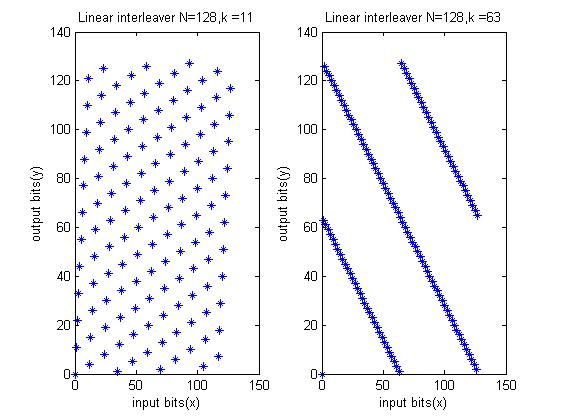
\includegraphics[width=\textwidth,keepaspectratio]{zemi2fig3.jpg}
\caption{Graphical representation of Linear interleaver with N=128, v=0 and k =[11,63]}
\label{}
\end{figure}

It can be seen that using an interger value closer to $sqrt(N)$ produces a lattice which is closer to that of a random interleaver. 


\newpage
\section{References}
\paragraph{[1]}  Oscar Y. Takeshita, Member, IEEE, and Daniel J. Costello ,''New Deterministic Interleaver Designs for Turbo Codes'',IEEE Trans. Inform. Theory, vol.  46,pp. 1988-2006,Nov. 2000\\
\paragraph{[2]}  L. C. Perez, J. Seghers, D. J. Costello, Jr., ''A distance spectrum interpretation of turbo codes'', IEEE Trans. Inform. Theory, vol. 42, pp. 1698-1709, Nov. 1996.\\
\paragraph{[3]} Jing Sun, Oscar Y. Takeshita ”Interleavers for Turbo Codes Using Permutation Polynomials over Integer Rings”, IEEE Trans. Inform. Theory, vol. 51,
pp. 101 - 119 Jan. 2005



\end{document}